%%=============================================================================
%% Methodologie
%%=============================================================================

\chapter{\IfLanguageName{dutch}{Methodologie}{Methodology}}
\label{ch:methodologie}

%% TODO: Hoe ben je te werk gegaan? Verdeel je onderzoek in grote fasen, en
%% licht in elke fase toe welke stappen je gevolgd hebt. Verantwoord waarom je
%% op deze manier te werk gegaan bent. Je moet kunnen aantonen dat je de best
%% mogelijke manier toegepast hebt om een antwoord te vinden op de
%% onderzoeksvraag.

\section{Performantie vergelijking}
Er zullen ter vergelijking verschillende testen uitgevoerd worden op elk apparaat. De testen die uitgevoerd zullen worden zijn een menu toevoegen, inloggen en een menu opzoeken met behulp van de filter.

\subsubsection{Gebruikte software}
\paragraph{Progressive web applicatie}
Het cypress pakket zorgt ervoor dat er verschillende UI testen kunnen uitgevoerd worden op een site, dit werd dan ook gebruikt omwille van de voorkeur van de developer.

\paragraph{Native applicatie}
Espresso wordt aangeraden voor de UI testen uit te voeren bij een native app, dit wordt ondersteund in android studio.

\subsubsection{Apparaten}
\paragraph{Progressive web applicatie}
Wegens dat de PWA testen niet kunnen uitgevoerd worden op een smartphone werden deze uitgevoerd op de Dell xps 15 9560. Aangezien de PWA dezelfde functionaliteiten kan uitvoeren met eenzelfde snelheid op een laptop en op de gemiddelde smartphone is dit een waardig alternatief.

\paragraph{Native applicatie}
De native applicatie testen werden uitgevoerd op de oneplus 5t, dit is een apparaat van 2017. Op deze wijze wordt er rekening gehouden met de gemiddelde smartphone van de bevolking.

\subsubsection{Vergelijking}
Om de applicaties met elkaar te vergelijken werden er een aantal functionaliteiten uitgevoerd. Deze zijn het ophalen van een menu en het weergeven van de detailpagina, en het filteren op de lijst pagina. De testen werden uitgevoerd op bovenstaande apparaten die steeds met hetzelfde draadloos netwerk verbonden waren om een zo goed mogelijke vergelijking te maken tussen de PWA en de Native applicatie.

%GRAFIEK DETAIL MENU TEST ALL
\begin{figure}[H]
	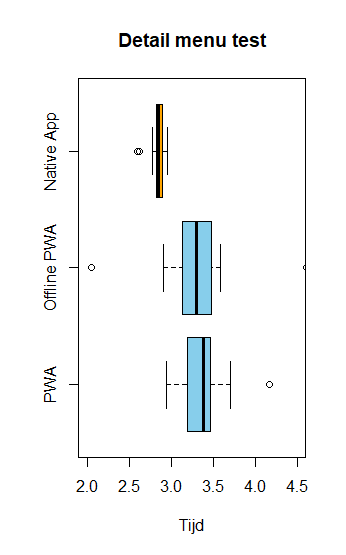
\includegraphics[width=200px]{Grafiek/Rplot_DetailMenu_AllType}\centering
	\caption{grafiek detail pagina test}
\end{figure}

\begin{table}[h!]
	\centering
	\begin{tabularx}{\textwidth }{|X|X|X|X|X|X|}
		\hline
		Type        & Min.  & 1ste Qu. & Gemiddelde & 3de Qu. & Max.  \\
		\hline
		PWA         & 2.940 & 3.205    & 3.380      & 3.465   & 4.170 \\
		\hline
		Offline PWA & 2.050 & 3.138    & 3.292      & 3.478   & 4.610 \\
		\hline
		Native App  & 2.596 & 2.826    & 2.846      & 2.901   & 2.952 \\
		\hline
	\end{tabularx}
	\label{table:1}
	\caption{Vergelijking van de performantie menu detail test}
\end{table}

Bovenstaande grafiek duidt aan dat een PWA er gemiddeld 3.38 seconden over doet om een menu op te halen en weer te geven. Dit is beduidend veel trager dan de native applicatie, vanwege de strategie die de PWA heeft. Tijdens deze testen moest de PWA voor elke pagina de styling ophalen samen met de data, hierdoor kan de PWA de laatste versie weergeven van de site. De native applicatie heeft een minder grote spreiding dan de PWA omdat deze niet afhankelijk is van de netwerkverbinding om de data weer te geven, aangezien de styling reeds gedownload is.

%GRAFIEK DEAIL MENU TEST PWA
\begin{figure}[H]
	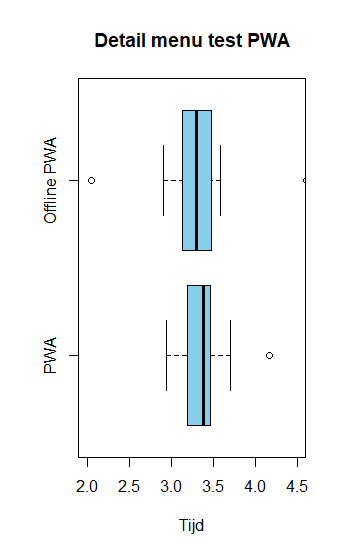
\includegraphics[width=200px]{Grafiek/Rplot_DetailMenu_PWA}\centering
	\caption{grafiek detail pagina test PWA}
\end{figure}

Eens de strategie veranderde naar cache-first deed de PWA er ongeveer even lang over  om de data op te halen, dit omdat er bij deze test geen onderscheid werd gemaakt tussen de applicatie in een offline of online status.

% GRAFIEK FILTER TEST
% GRAFIEK FILTER TEST PWA
\begin{figure}[H]
	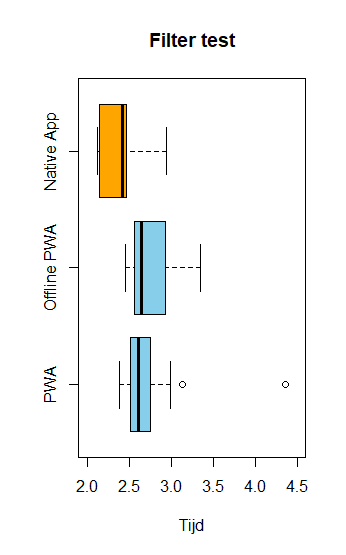
\includegraphics[width=200px]{Grafiek/Rplot_Filter_AllType}\centering
	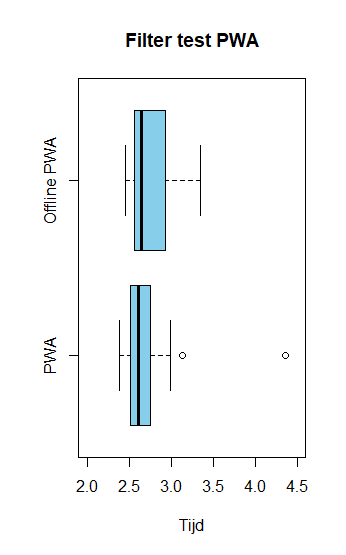
\includegraphics[width=200px]{Grafiek/Rplot_Filter_PWA}\centering
	\caption{grafiek menu filter test}
\end{figure}

\begin{table}[h!]
	\centering
	\begin{tabularx}{\textwidth }{|X|X|X|X|X|X|}
	\hline
		Type        & Min.  & 1ste Qu. & Gemiddelde & 3de Qu. & Max.  \\
	\hline
		PWA         & 2.380 & 2.522    & 2.693      & 2.745   & 4.360 \\
	\hline
		Offline PWA & 2.460 & 2.565    & 2.752      & 2.992   & 3.350 \\
	\hline
		Native App  & 2.118 & 2.152    & 2.360      & 2.474   & 2.950 \\
	\hline
	\end{tabularx}
	\label{table:2}
	\caption{Vergelijking van de performantie menu detail test}
\end{table}

Bovenstaande grafiek indiceert dat de PWA eveneens trager is dan de native applicatie. Opvallend is dat de offline strategie van de PWA een grotere spreiding heeft van resultaten dan de online strategie. Dit is merkwaardig aangezien de offline PWA eerst naar de cache kijkt vooraleer dat er een online data bevraging plaatsvindt.

\section{Benodigde ruimte}
De benodigde ruimte werd opgevraagd direct na de installatie en na het openen van de applicatie, dit omdat de applicatie nog geen extra gecachte data heeft als deze pas gedownload is. 

%GRAFIEK BENODIGDE RUIMTE NO CACHED
\begin{figure}[h]
	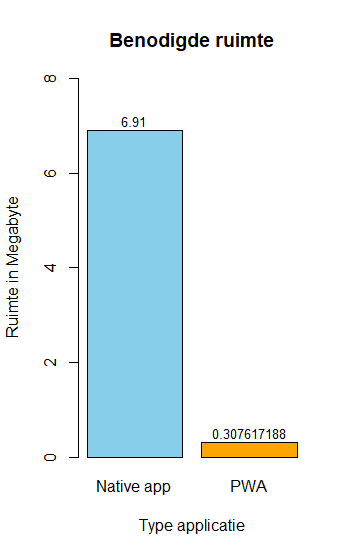
\includegraphics[width=200px]{Grafiek/Rplot_BenodigdeRuimte_PWANativeApp_NoCached}\centering
	\caption{grafiek benodigde ruimte geen cache}
\end{figure}

\begin{table}[h!]
	\centering
	\begin{tabular}{|c|c|}
		\hline
		Type              & Benodigde ruimte \\
		\hline
		PWA               & 0.307619188      \\
		\hline
		Native applicatie & 6.91             \\
		\hline
	\end{tabular}
	\label{table:3}
	\caption{Benodigde ruimte applicatie geen cache}
\end{table}
In bovenstaande grafiek ziet u een duidelijk verschil tussen de progressive web app en de native applicatie. De native applicatie neemt 95.55\% meer plaats in ten opzichte van de progressive web applicatie. Een native applicatie heeft het nadeel dat de styling al wordt meegegeven tijdens de installatie, bij een PWA is dit niet zo.

% GRAFIEK BENODIGDE RUIMTE CACHED
\begin{figure}[H]
	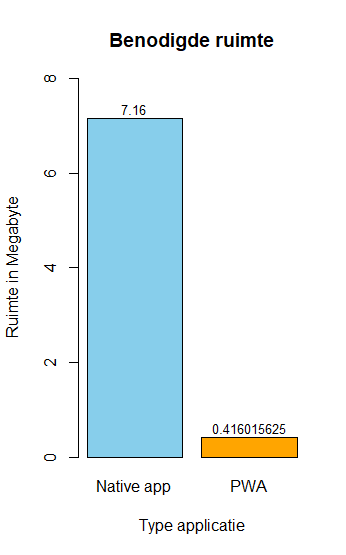
\includegraphics[width=200px]{Grafiek/Rplot_BenodigdeRuimte_PWANativeApp_Cached}\centering
	\caption{grafiek benodigde ruimte met cache}
\end{figure}

\begin{table}[h!]
	\centering
	\begin{tabular}{|c|c|}
		\hline
		Type              & Benodigde ruimte \\
		\hline
		PWA               & 0416015625       \\
		\hline
		Native applicatie & 7.16             \\
		\hline
	\end{tabular}
	\label{table:4}
	\caption{Benodigde ruimte applicatie met cache}
\end{table}
In bovenstaande grafiek is het duidelijk dat een PWA veel minder ruimte in neemt dan een native applicatie, zelfs na het ophalen van alle data.

% GRAFIEK BENODIGDE RUIMTE PWA
\begin{figure}[H]
	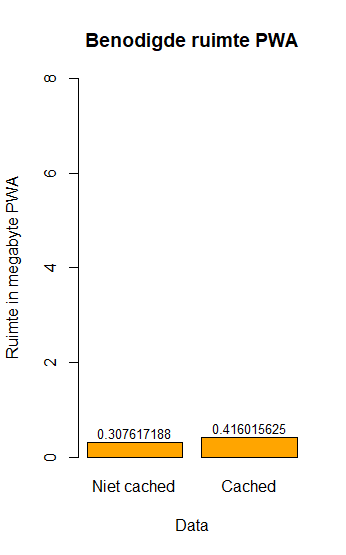
\includegraphics[width=200px]{Grafiek/Rplot_BenodigdeRuimte_PWA}\centering
	\caption{grafiek benodigde ruimte PWA}
\end{figure}

\begin{table}[h!]
	\centering
	\begin{tabular}{|c|c|}
		\hline
		Data              & Benodigde ruimte \\
		\hline
		Niet cached       & 0.307617188       \\
		\hline
		Cached            & 0.416015625       \\
		\hline
	\end{tabular}
	\label{table:5}
	\caption{Benodigde ruimte PWA}
\end{table}

De PWA neemt wel 35.24\% meer plaats in nadat de data gecached is. Dit omdat de PWA pas de styling en data opvraagt eens de applicatie voor een eerste keer opgestart is. Nadien wordt de data opnieuw opgehaald eens de pagina opnieuw geladen wordt door de gebruiker of na het lanceren van de applicatie.

%GRAFIEK BENODIGDE RUIMTE NATIVE APP
\begin{figure}[H]
	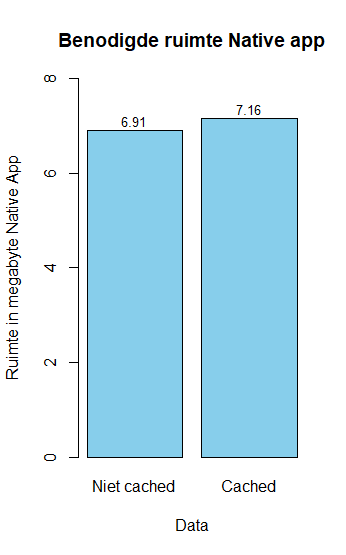
\includegraphics[width=200px]{Grafiek/Rplot_BenodigdeRuimte_NativeApp}\centering
	\caption{grafiek benodigde ruimte native applicatie}
\end{figure}

\begin{table}[h!]
	\centering
	\begin{tabular}{|c|c|}
		\hline
		Data             & Benodigde ruimte \\
		\hline
		Niet cached       & 6.91             \\
		\hline
		Cached            & 7.16             \\
		\hline
	\end{tabular}
	\label{table:6}
	\caption{Benodigde ruimte native applicatie}
\end{table}

De native applicatie cached enkel de data die deze nodig heeft omdat de styling van de applicatie meegegeven wordt tijdens de installatie. Om die reden is er maar een verschil van 3.62\% in bestandsgrootte.

\section{Gebruikerservaring}
Wegens het coronavirus konden verschillende proefpersonen niet deelnemen aan dit onderzoek. Om deze reden is dit onderzoek uitgevoerd in een dichtere omgeving met iets meer technisch vaardige personen. Er werd gevraagd aan de proefpersonen om verschillende taken uit te voeren op de applicatie, deze waren de volgende. Er werd aan elk van hen gevraagd om een menu te genereren, een menu toe te voegen, een menu te verwijderen en een menu op te vragen aan de hand van een filter. Tijdens deze testen werd ook gevraagd om hun gedachtengang luidop mee te delen, dit omdat het zo duidelijk is voor alle partijen zodat de proefpersoon zich kan navigeren door de applicatie.

\subsubsection{Native applicatie}
Eén proefpersoon had geen ondersteuning op het apparaat omwille van een te lage android versie, deze proefpersoon kon wel de PWA applicatie installeren.

%HOMESHCERM NATIVE
\begin{figure}[H]
	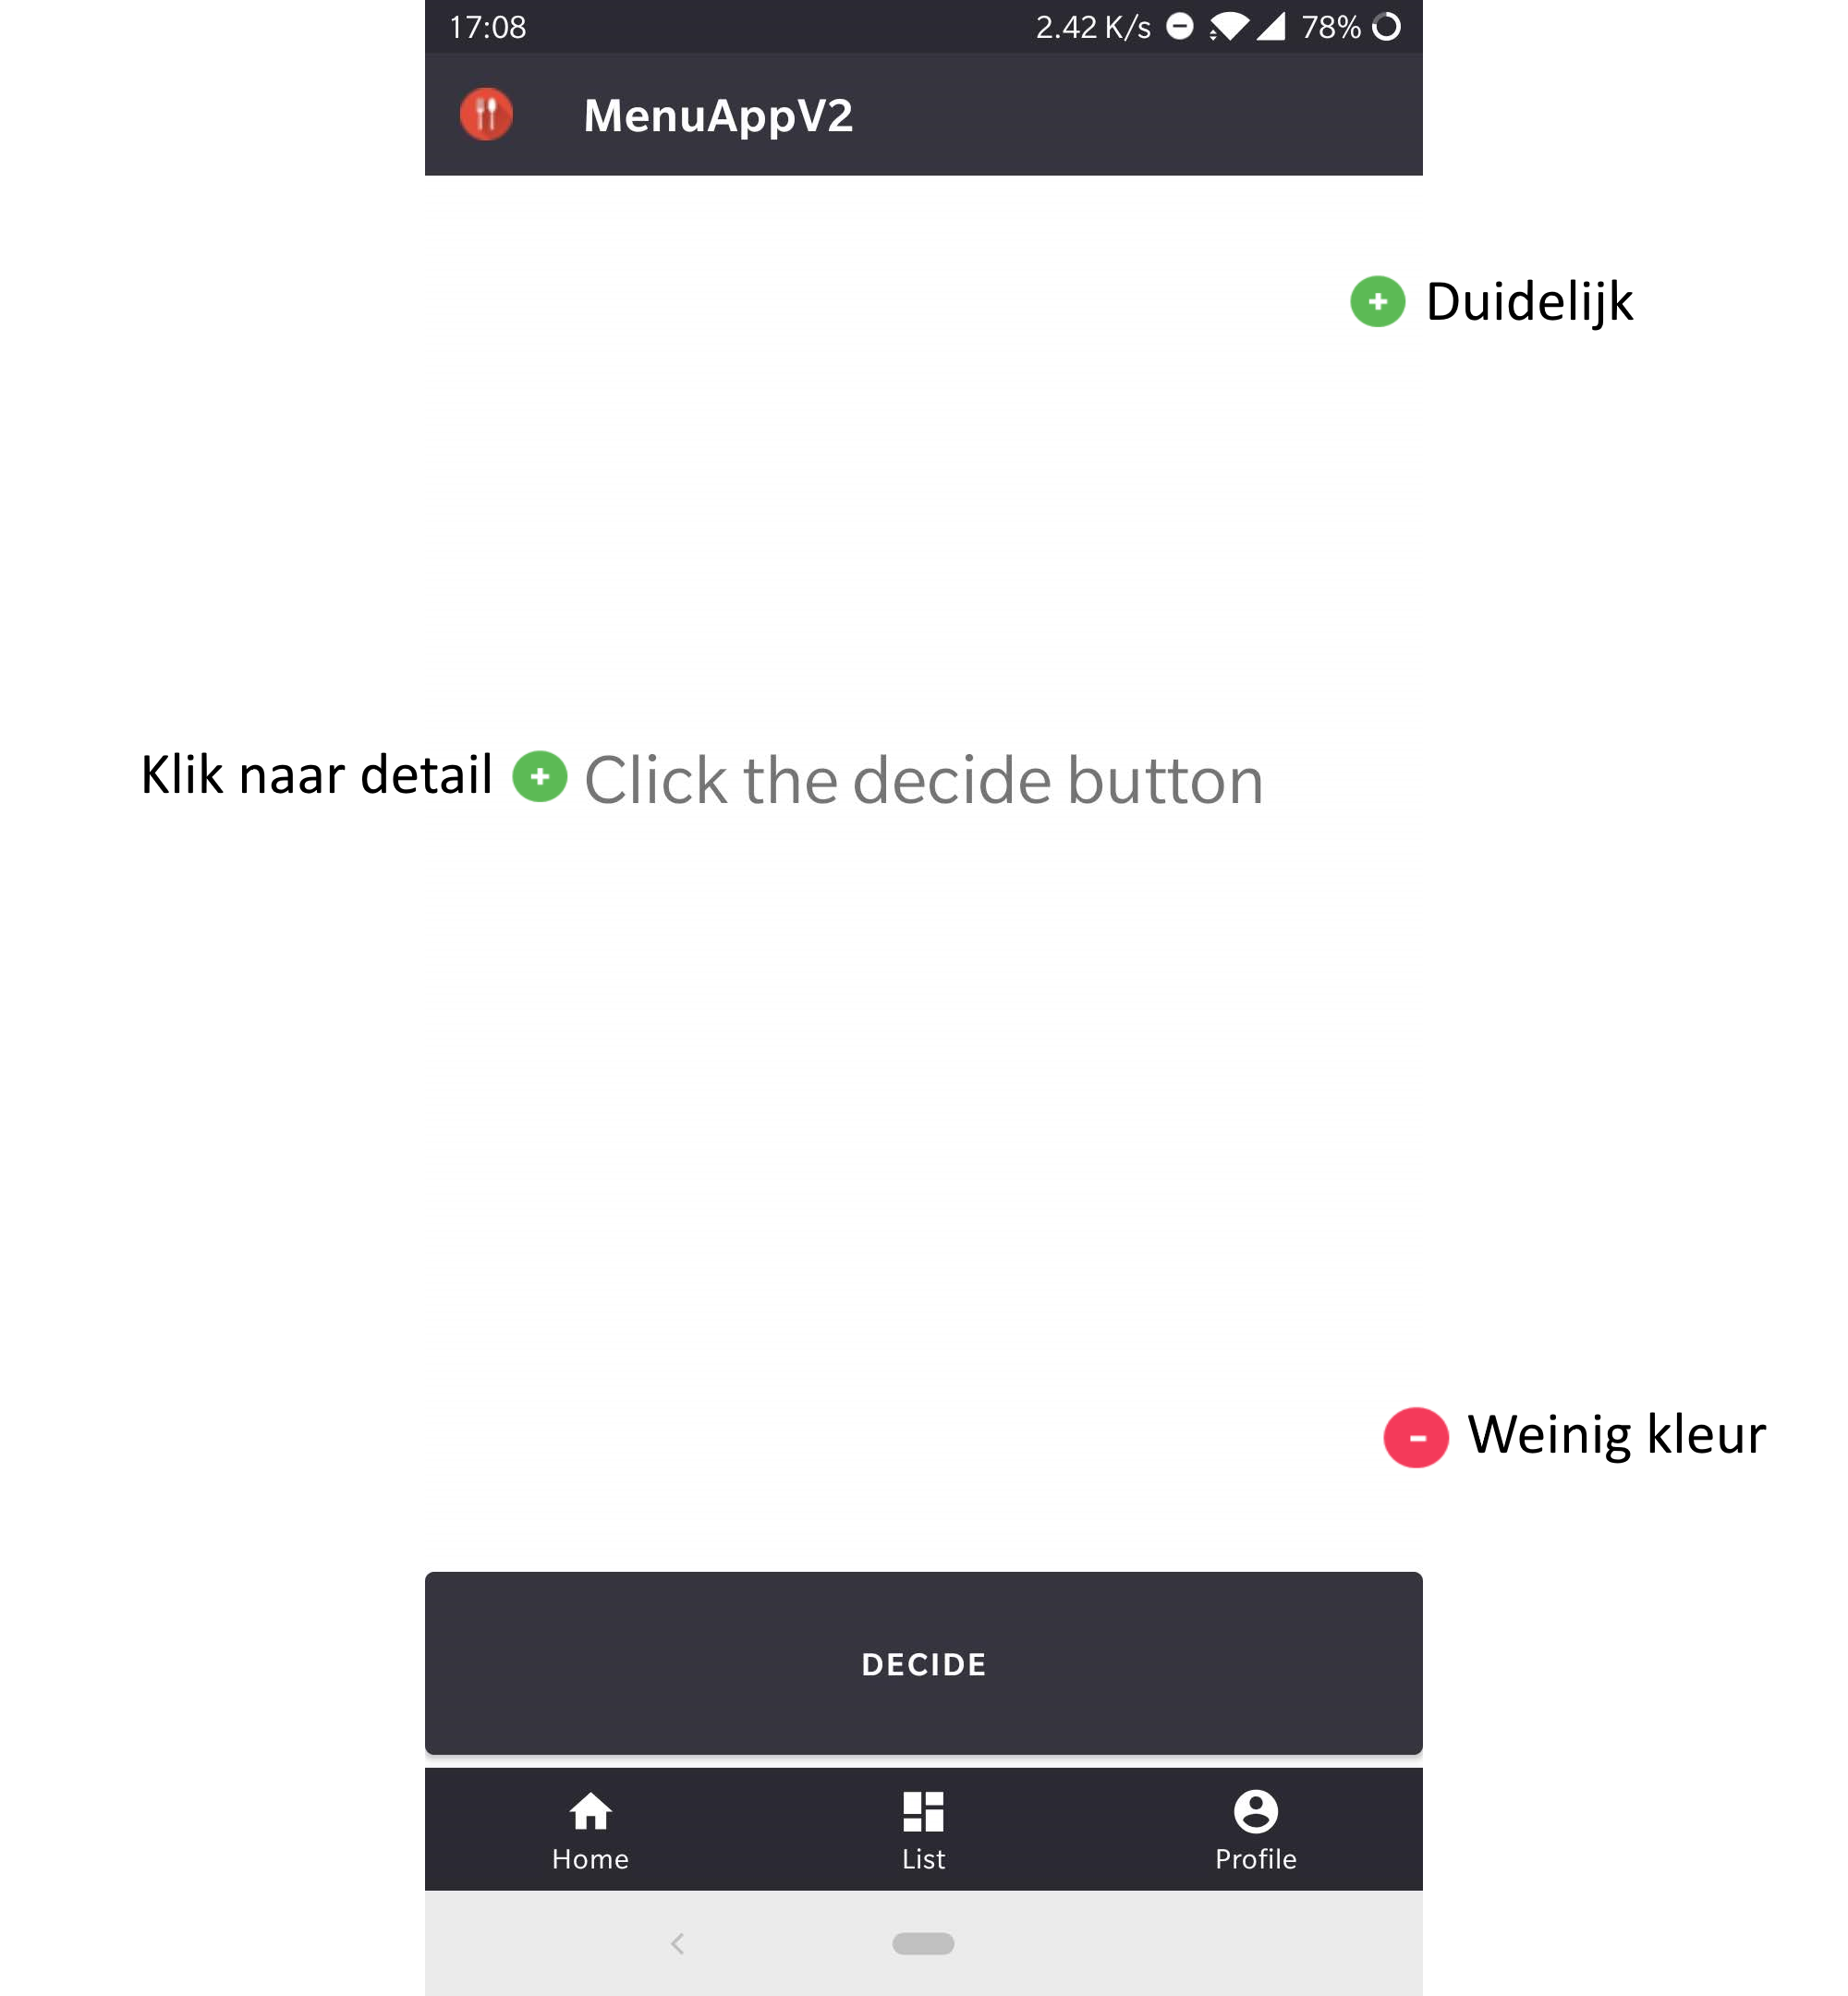
\includegraphics[width=200px]{Screenshot/App/App_Homescherm}\centering
	\caption{homescherm native applicatie}
\end{figure}
Op het homescherm kwam er de opmerking dat er weinig kleur gebruikt werd maar dat het wel duidelijk was. De proefpersonen vonden het ook handig dat je kon doorklikken op de titel van het gegenereerde menu.

%DETAIL PAGINA
\begin{figure}[H]
	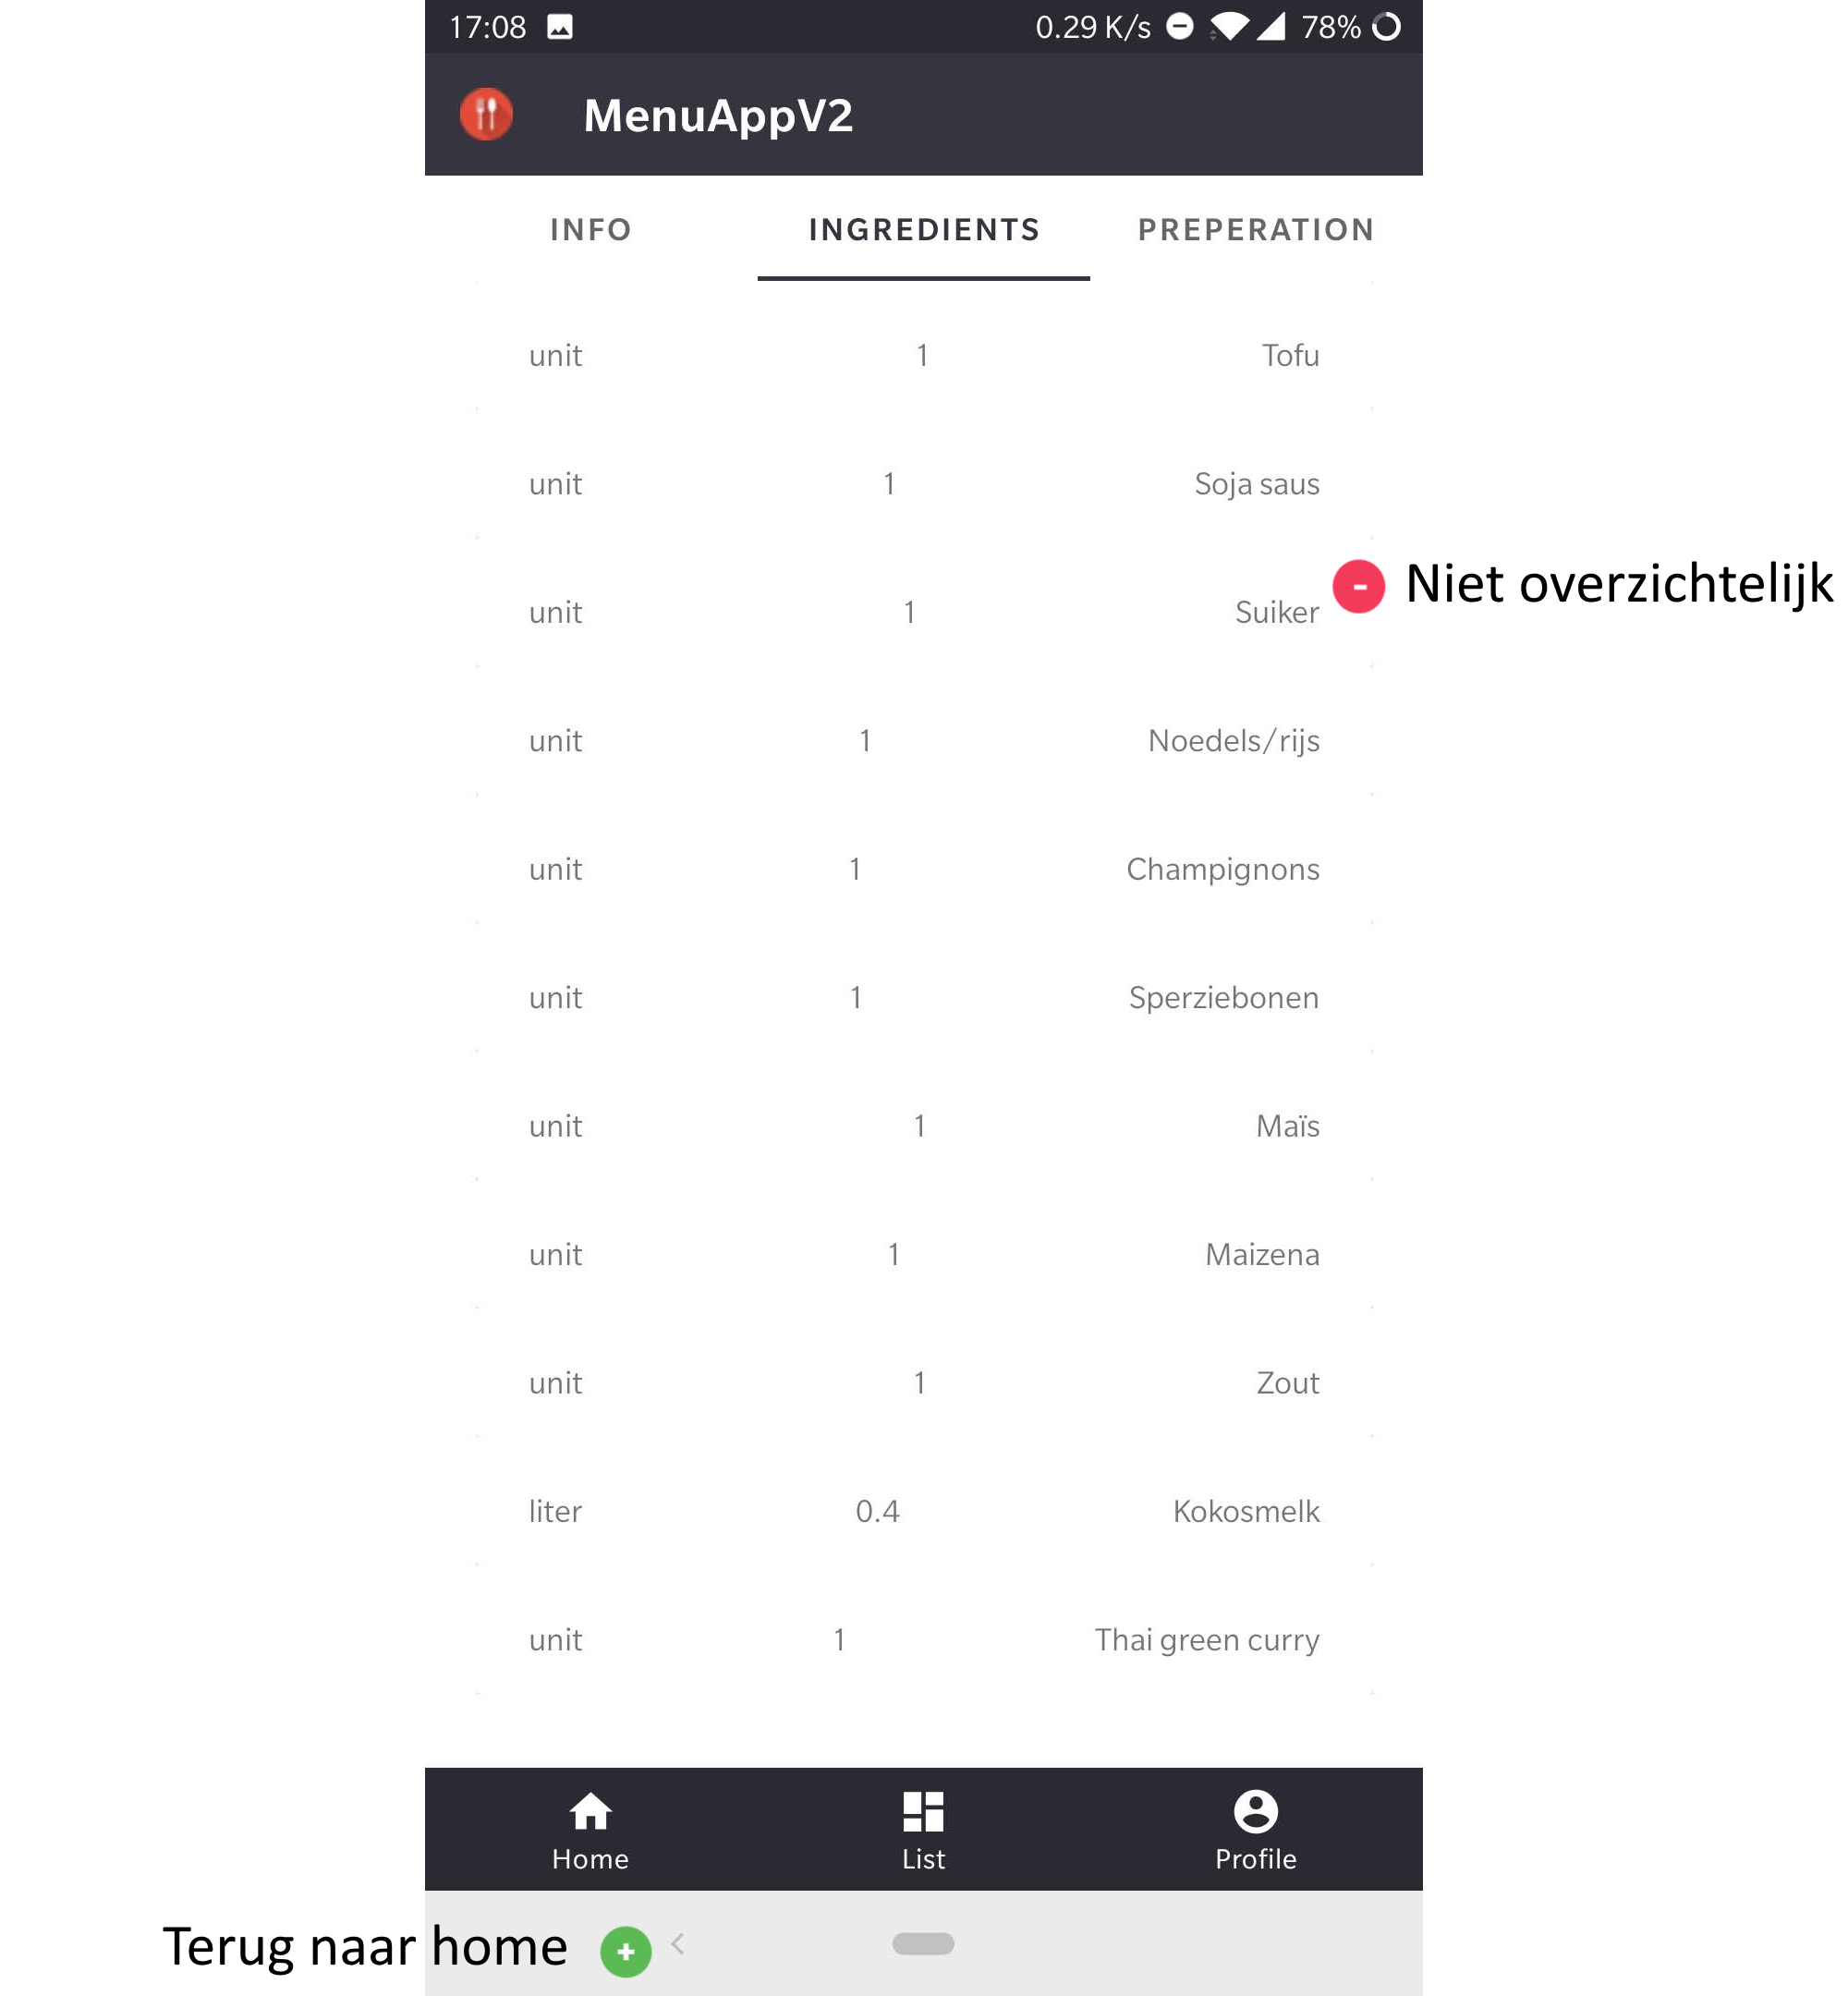
\includegraphics[width=200px]{Screenshot/App/App_Detail}\centering
	\caption{menu detail pagina native applicatie}
\end{figure}
Op de detailpagina werden er de opmerkingen gegeven dat het niet overzichtelijk is omwille van de indeling van de pagina en omdat de hoeveelheden niet onder elkaar staan. Wat de gebruikers wel positief vonden is dat je direct terug kan gaan naar de homepagina zonder eerst naar alle aangeduide tabs terug te gaan.

%VOORBEREIDING NATIVE
\begin{figure}[H]
	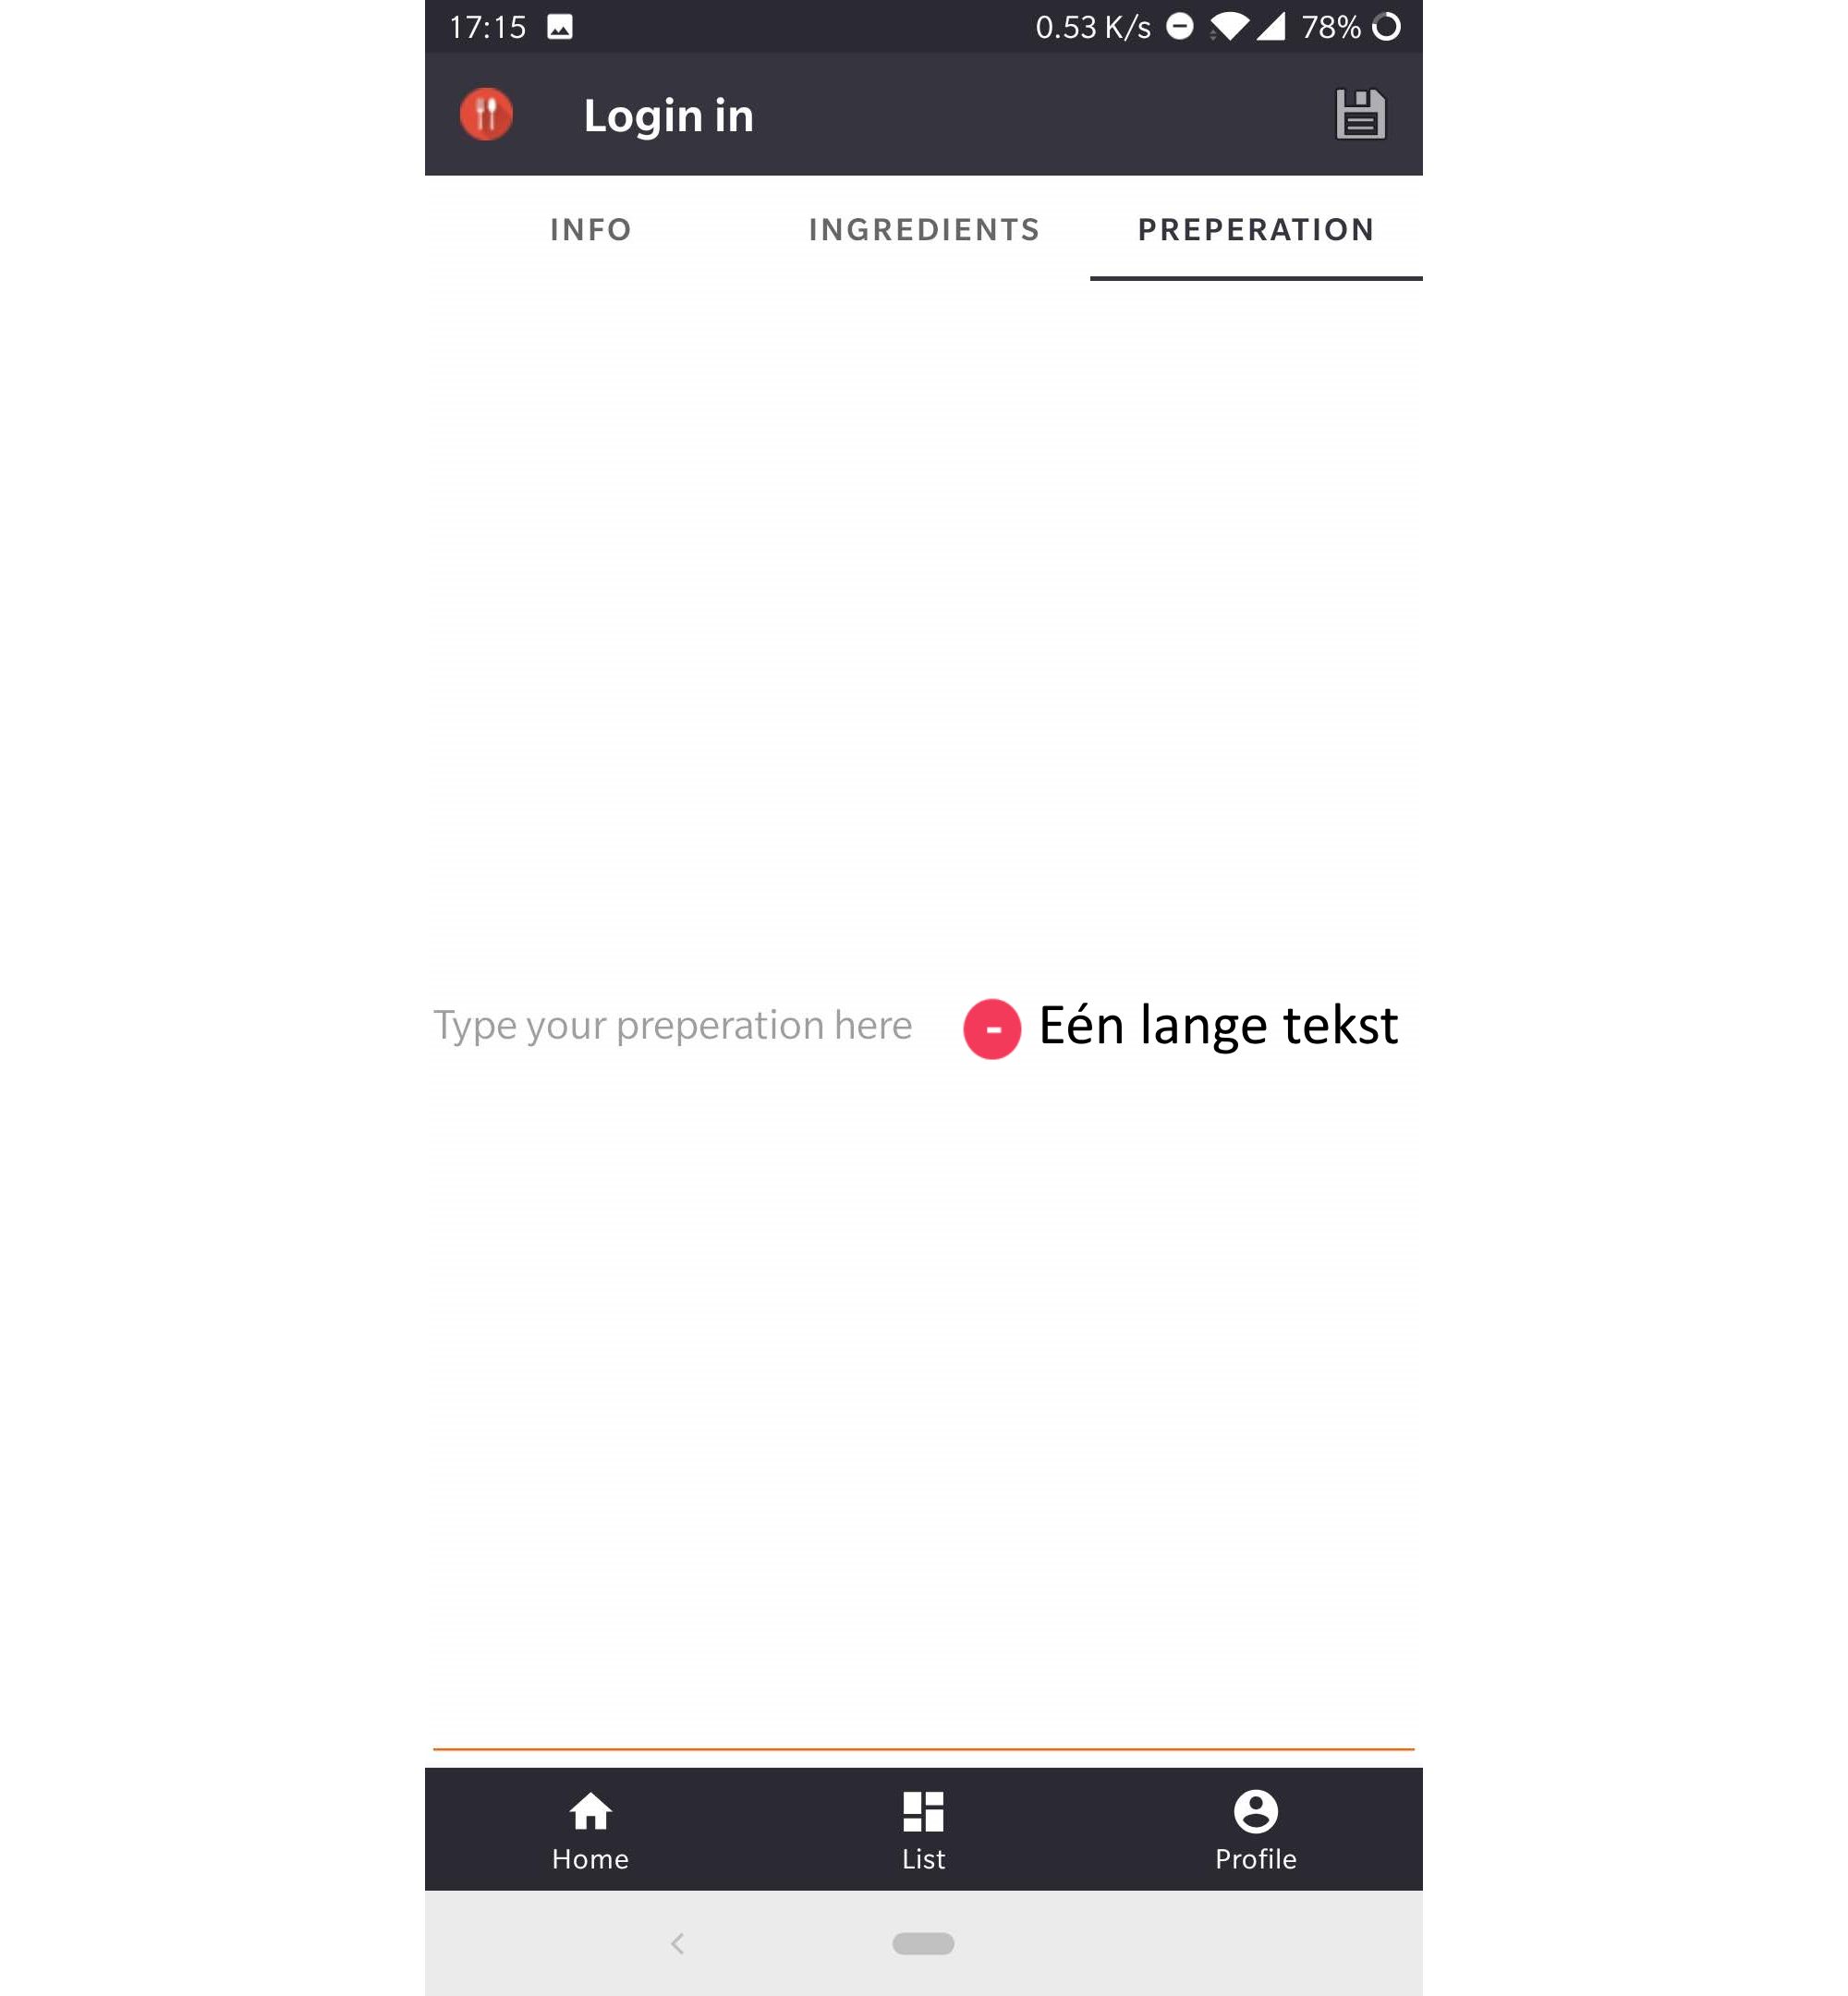
\includegraphics[width=200px]{Screenshot/App/App_Perperation}\centering
	\caption{menu voorbereiding pagina native applicatie}
\end{figure}
Tijdens het invullen van de voorbereiding werd er getwijfeld wat er moest ingevuld worden, dit omdat er één grote tekstbox is die niet in stappen onderverdeeld is.

%LOGIN NATIVE
\begin{figure}[H]
	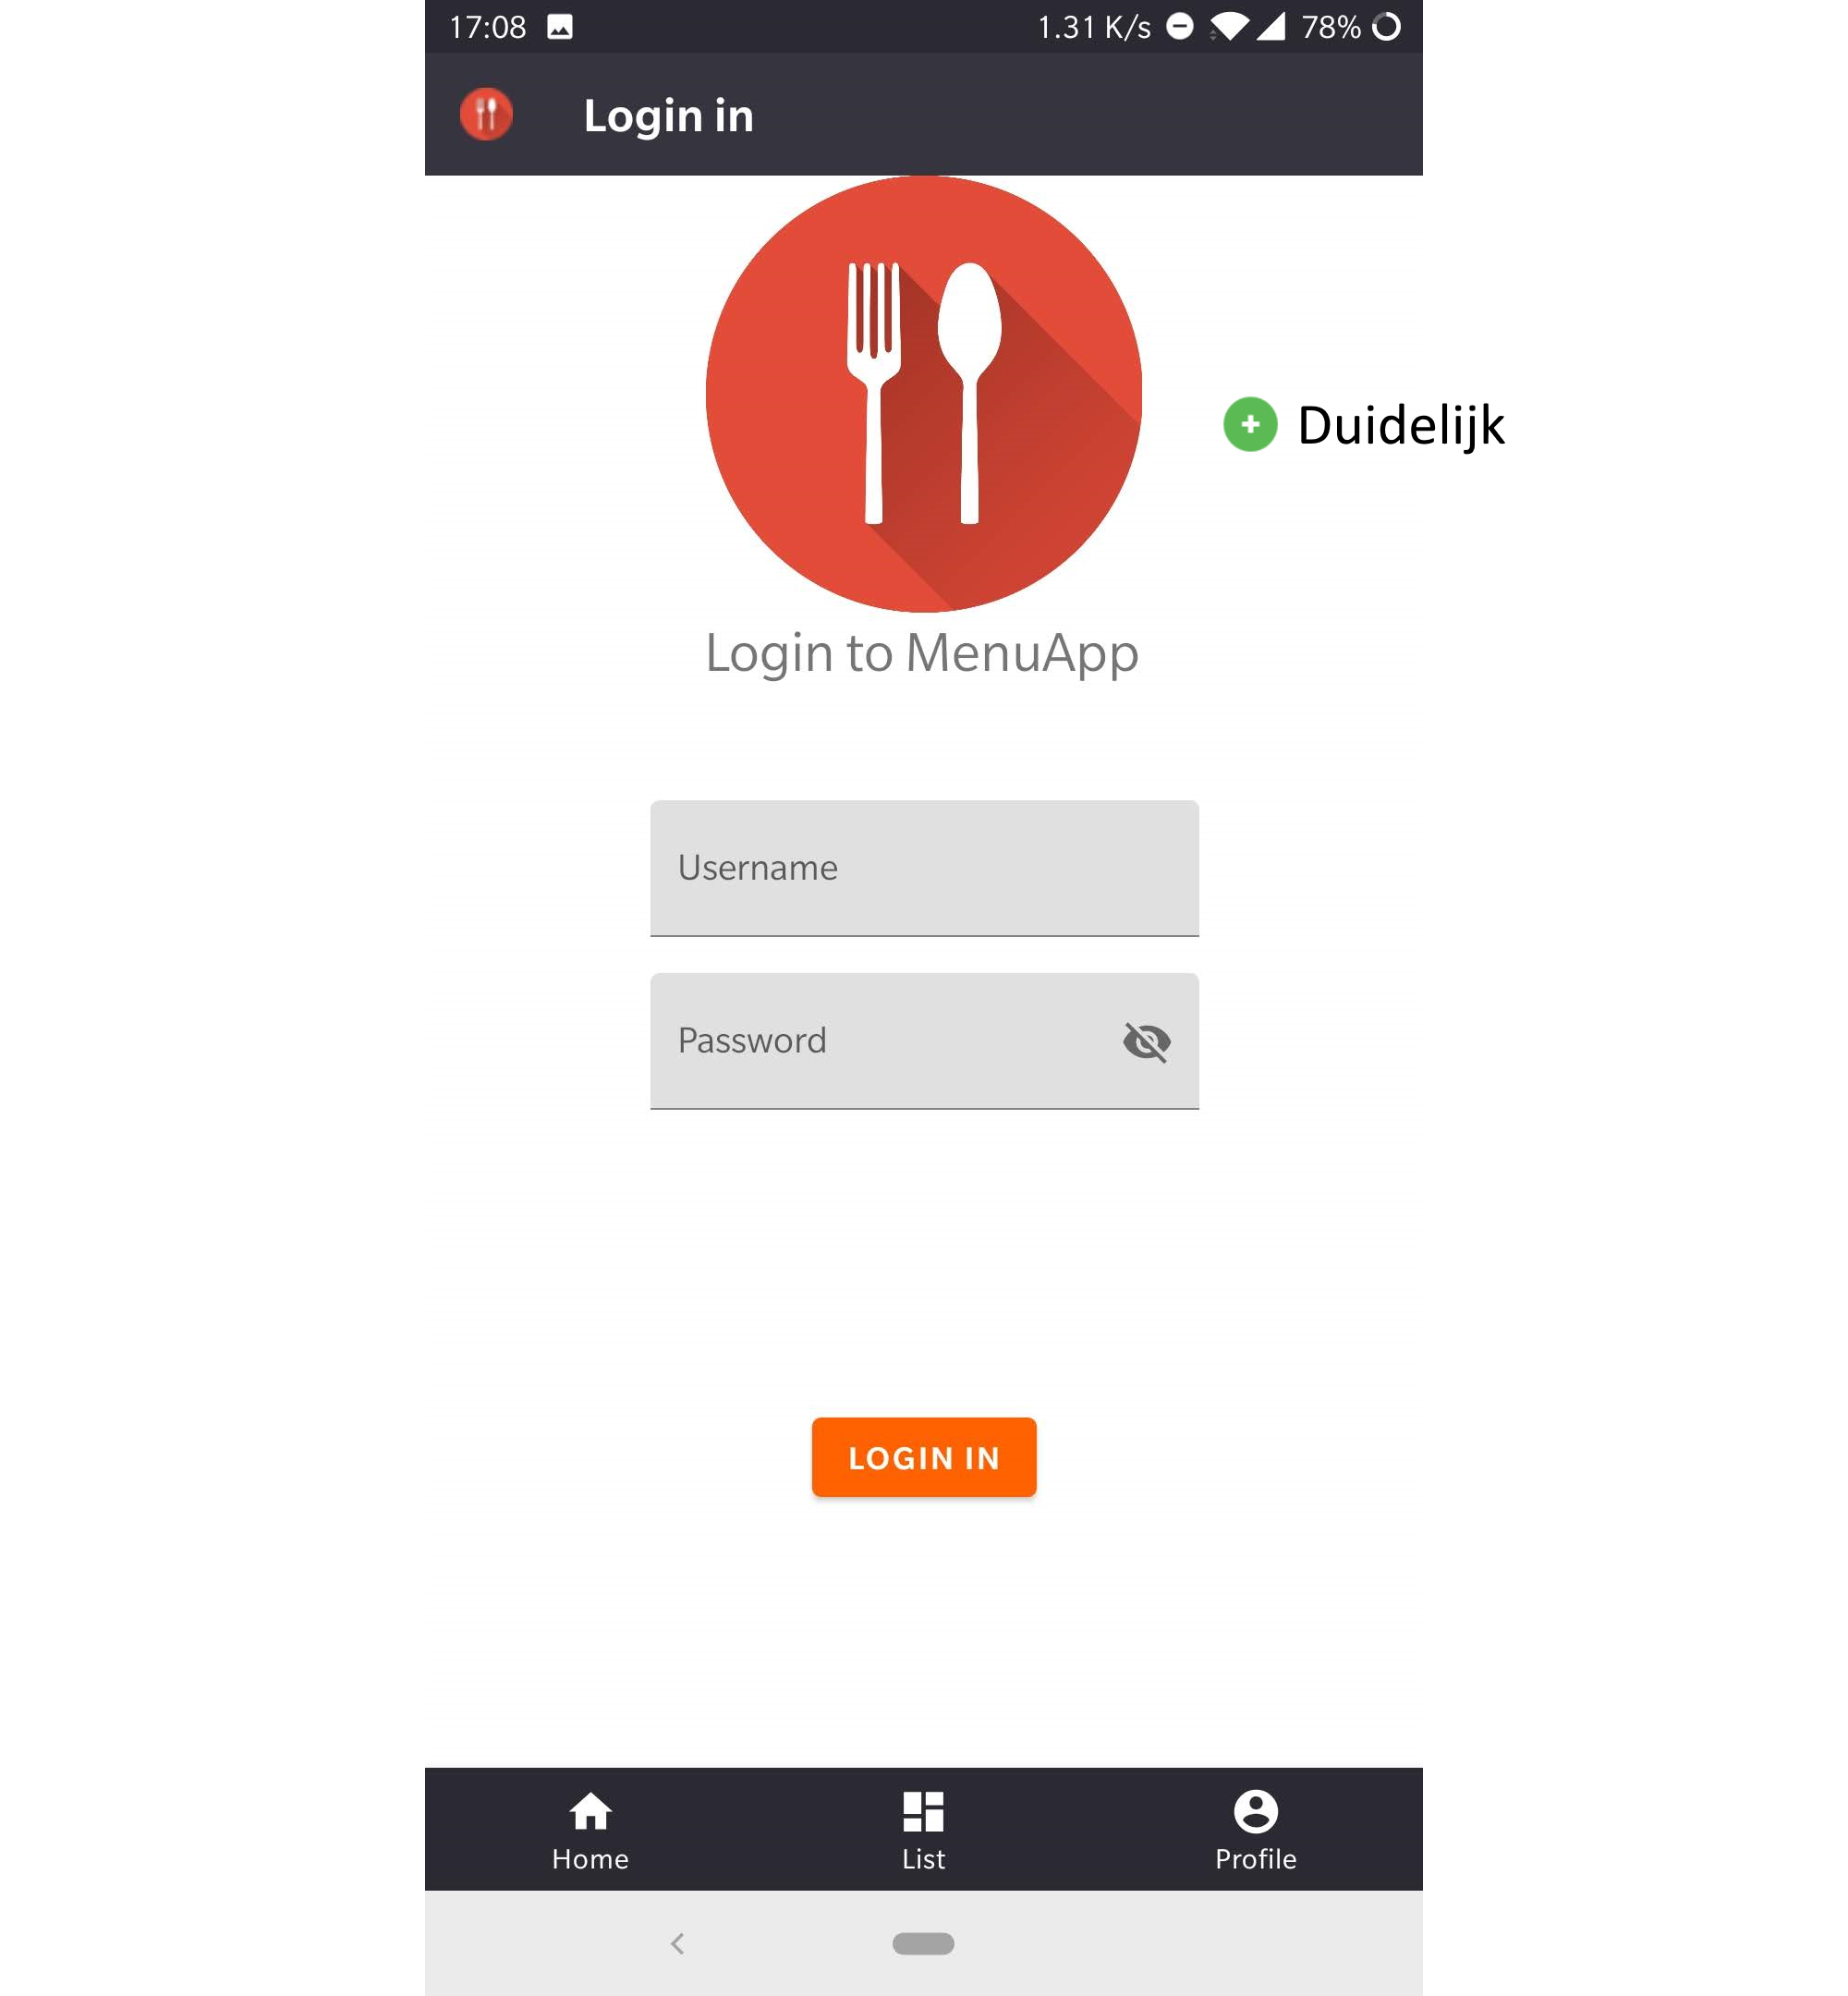
\includegraphics[width=200px]{Screenshot/App/App_Login}\centering
	\caption{login pagina native applicatie}
\end{figure}
De login pagina was heel duidelijk en volgens sommige gebruikers wel aantrekkelijk.

\subsubsection{Progressive web applicatie}
Voor de installatie van de PWA hadden de meeste testpersonen externe hulp nodig omdat dit niet even gebruiksvriendelijk is als de traditionele app store. De proefpersonen gaven aan dat een melding wel handig was geweest zodat het duidelijker was dat deze site als applicatie beschikbaar was.

%HOMEPAGE PWA
\begin{figure}[H]
	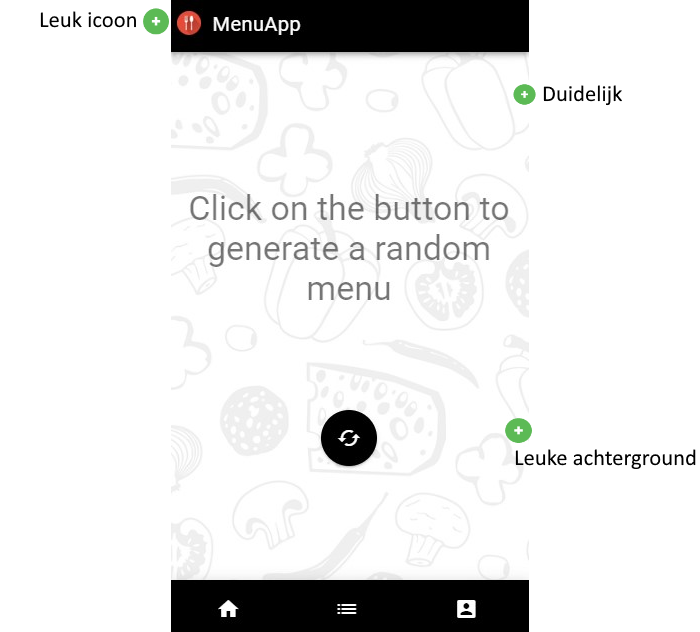
\includegraphics[width=200px]{Screenshot/Site/Site_homepage}\centering
	\caption{home pagina PWA}
\end{figure}
Op de homepagina werden er vooral opmerkingen gegeven over de indeling ervan. Over het algemeen werd de homepagina wel als duidelijk beschouwd door de proefpersonen.

%FILTER PAGE PWA
\begin{figure}[H]
	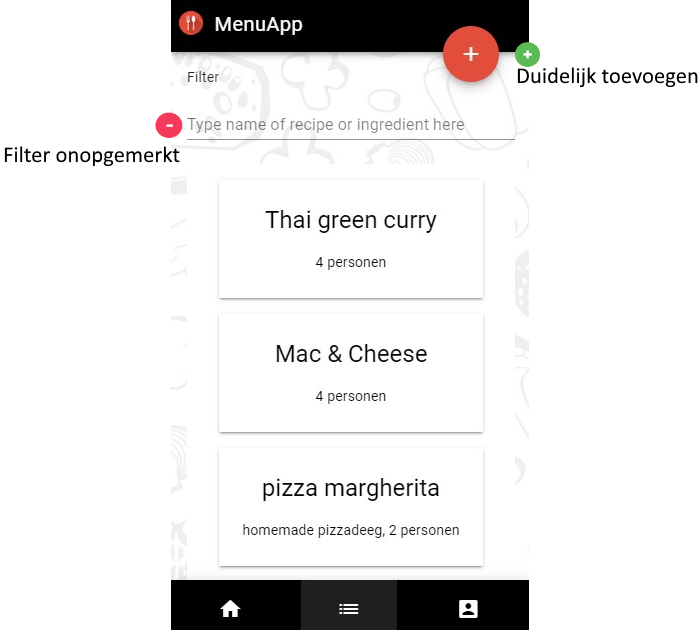
\includegraphics[width=200px]{Screenshot/Site/Site_listpage}\centering
	\caption{filter pagina PWA}
\end{figure}
Op de overzichtspagina werd de filter niet opgemerkt totdat we de proefpersoon vroegen om iets op te zoeken, verschillende proefpersonen zochten hierbij gewoon in de lijst. De proefpersonen gaven ook aan dat de filter duidelijker was op de app omdat deze daar groter staat. Het is wel duidelijk dat de grote plus bovenaan er staat om een recept toe te voegen.

%INGREDIENTS PAGE PWA
\begin{figure}[H]
	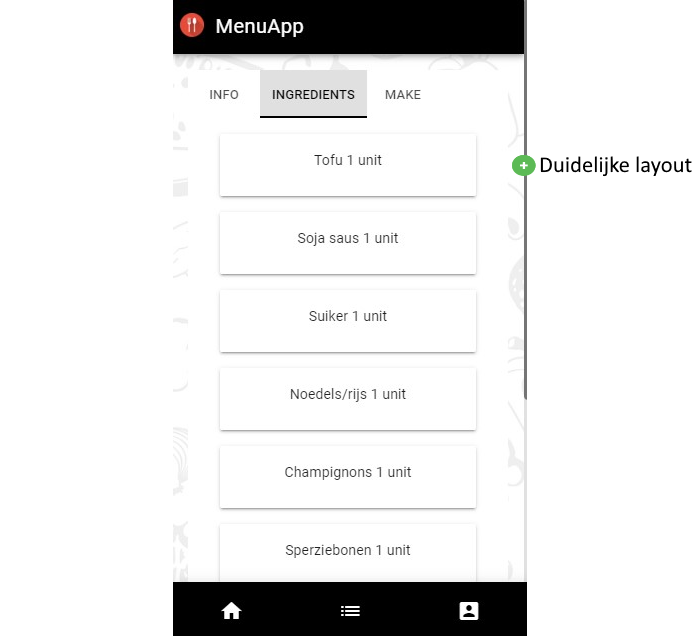
\includegraphics[width=200px]{Screenshot/Site/Site_detail_ingredients}\centering
	\caption{menu ingredienten pagina PWA}
\end{figure}
Op de detailpagina was alles duidelijk volgens de proefpersonen. Er werd wel de opmerking gegeven dat je niet direct terug gaat naar het home scherm met de terug knop.

%ADD MENU INGREDINETS PWA
\begin{figure}[H]
	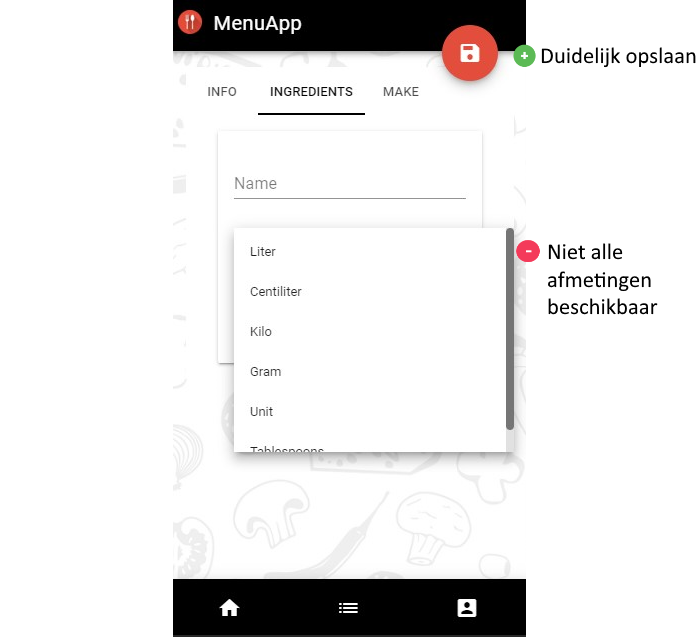
\includegraphics[width=200px]{Screenshot/Site/Site_addMenu_ingredients}\centering
	\caption{menu toevoegen ingredienten pagina PWA}
\end{figure}
De proefpersonen hadden geen probleem met het aanmaken van de ingrediënten. Er waren wel enkele opmerkingen over hoe de menu precies geïmplementeerd moesten worden zoals bij de voorbereiding, dit omdat de voorbereiding één groot tekstveld is.

%LOGIN PWA
\begin{figure}[H]
	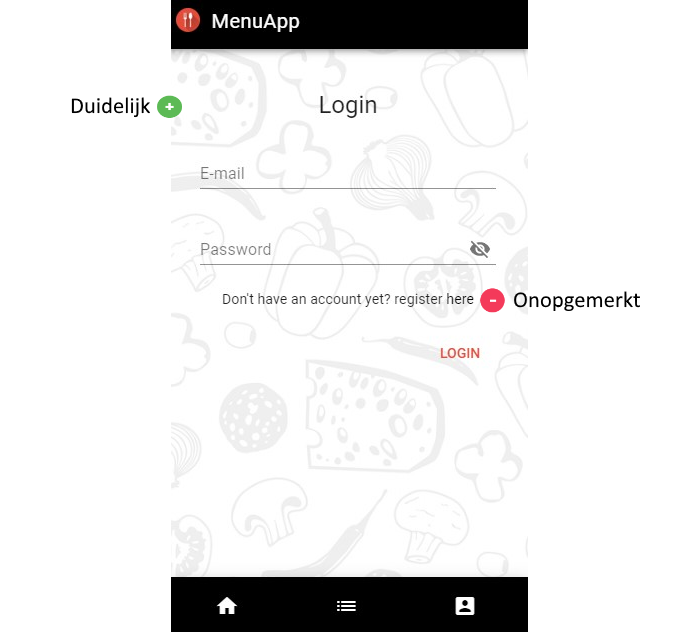
\includegraphics[width=200px]{Screenshot/Site/Site_Login}\centering
	\caption{login pagina PWA}
\end{figure}
Het login scherm was voor de proefpersonen redelijk duidelijk, sommige proefpersonen hadden wel wat moeite om de registratiepagina te vinden.